%%%%%%%%%%%%%%%%%%%%%%%%%%%%%%%%%%%%%%%%%
% FRI Data Science_report LaTeX Template
% Version 1.0 (28/1/2020)
% 
% Jure Demšar (jure.demsar@fri.uni-lj.si)
%
% Based on MicromouseSymp article template by:
% Mathias Legrand (legrand.mathias@gmail.com) 
% With extensive modifications by:
% Antonio Valente (antonio.luis.valente@gmail.com)
%
% License:
% CC BY-NC-SA 3.0 (http://creativecommons.org/licenses/by-nc-sa/3.0/)
%
%%%%%%%%%%%%%%%%%%%%%%%%%%%%%%%%%%%%%%%%%


%----------------------------------------------------------------------------------------
%	PACKAGES AND OTHER DOCUMENT CONFIGURATIONS
%----------------------------------------------------------------------------------------
\documentclass[fleqn,moreauthors,10pt]{ds_report}
\usepackage[english]{babel}

\graphicspath{{fig/}}




%----------------------------------------------------------------------------------------
%	ARTICLE INFORMATION
%----------------------------------------------------------------------------------------

% Header
\JournalInfo{FRI Natural language processing course 2025}

% Interim or final report
\Archive{Project report} 
%\Archive{Final report} 

% Article title
\PaperTitle{'; DROP TABLE TEAMS; --} 

% Authors (student competitors) and their info
\Authors{Henri Sellis, Igor Sitek}

% Advisors
\affiliation{\textit{Advisors: Aleš Žagar}}

% Keywords
\Keywords{Retrieval-Augmented Generation, RAG, web scraping, rank algorithms, Python, keyword extraction}
\newcommand{\keywordname}{Keywords}


%----------------------------------------------------------------------------------------
%	ABSTRACT
%----------------------------------------------------------------------------------------

\Abstract{
For our Natural Language Processing course group project, we are developing a conversational agent that retrieves additional information from Google Scholar documents, to increase the quality of answering questions, ensuring up-to-date outputs. To accomplish this, first a number of most relevant keywords are extracted from the user input, then corresponding queries are made to retrieve documents from Google Scholar, and finally the documents, alongside with the original user input, are passed to a Large Language Model, to generate a paraphrased response.
}

%----------------------------------------------------------------------------------------

\begin{document}

% Makes all text pages the same height
\flushbottom 

% Print the title and abstract box
\maketitle 

% Removes page numbering from the first page
\thispagestyle{empty} 

%----------------------------------------------------------------------------------------
%	ARTICLE CONTENTS
%----------------------------------------------------------------------------------------

\section*{Introduction}
	Large Language Models have proven to be very successful at general-knowledge topics, but a trained model cannot continuously stay up to date with the most recent academic topics. To solve this problem, we are using Retrieval-Augmented Generation to provide an LLM with the most relevant academic papers to allow the LLM to generate more relevant and accurate responses. The documents are retrieved from Google Scholar, as it is an easily accessible repository with lots of academic papers.
	
	With the increasing number of scientific papers published across the world, it is difficult to analyze the most relevant data. Automated literature lookup based on relevant datasets might highly improve the process of conducting scientific experiments, mitigating the risk of work duplication. However, it is crucial to ensure up-to-date answers, thus relying on static datasets is not the most optimal approach. RAG-augmented query analyses alongside with web crawling and web scraping techniques seem to be promising to resolve that matter.


%------------------------------------------------

\section*{Methodology}

\begin{figure}[ht]\centering 
	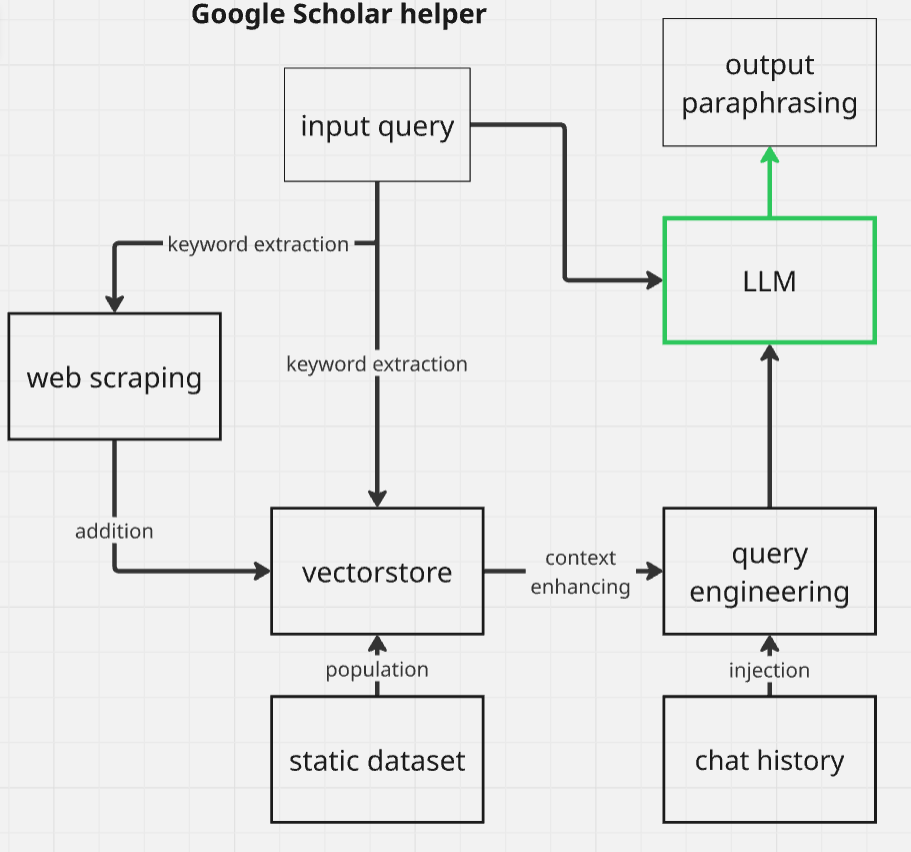
\includegraphics[width=\linewidth]{images/scheme.png}
	\caption{\textbf{System scheme} High-level overview of chat-bot system proposed in this paper.}
	\label{fig:scheme}
\end{figure}

The proposed methodology scheme is presented in figure~\ref{fig:scheme}. Each vital step is described in the following subsections of this article.

\subsection*{Corpus analysis}

To specify our domain, we will limit our research to English papers only, eliminating the necessity of language-independent vector transitions and specific rules in different languages. The English language was chosen as it is the most popular language with the highest amount of data available, and it is characterized by low sentence sensitivity (in opposition to romance languages). That characteristic enables low-effort word stemming in text processing~\cite{turney2000learning}.

\subsection*{Keyword extraction}

In order to be able to query for relevant literature, keywords need to be extracted from user input. These keywords can be used as a Google Scholar query.

Work ~\cite{siddiqi2015keyword} is a review of existing methods for keyword extraction, containing summaries of different supervised and unsupervised algorithms. Upon these, Neural Networks seem to be used mainly. On the other hand, ready-to-use implementations of RAKE and RANK algorithms (like TextRank~\cite{textrank} - https://github.com/davidadamojr/TextRank or TopicRank~\cite{bougouin2013topicrank} - https://github.com/Aayushpatel007/topicrankpy) seem to be useful enough for our case. Due to simplicity of use, the KeyBERT model \cite{grootendorst2020keybert} was chosen. It uses BERT-embeddings and simple cosine similarity to find the most central sub-phrases in a text.

\subsection*{Web scraping}

Keywords extracted from user input are combined into a suitable Google Scholar query, in order to find the most relevant academic documents which might include useful context for the chatbot for answering the user's question. Querying Google Scholar was implemented using the Scholarly \cite{cholewiak2021scholarly} library.

However, many of the documents findable in Google Scholar are not directly downloadable. To solve this issue, we implemented a secondary functionality for downloading the found papers from SciHub \cite{scihub}, when they are not directly available from Google Scholar. 

\subsection*{Document retrieval}

After online paper scraping, all documents are split into chunks and kept in a FAISS \textit{vectorstore}. Based on the similarity indicator within the configured threshold, the most relevant documents are provided for further use. These are then filtered out using a re-ranking algorithm for double-check safety and context sanity.

\subsection*{Static dataset}

In order to avoid starting from a completely empty FAISS vectorstore, a dataset of science papers \cite{rncamposgithub} was processed and added into the vectorstore, in the same way as described in the previous paragraph.

The dataset consists of zip folders with two sub-folders, one containing whole papers in TXT format, and one with manually gathered keywords and key-phrases. These files are matched based on a common key - included in the filename.

\subsection*{Data combining and paraphrasing}

All the relevant documents (found in the static dataset and downloaded from the web) are combined with user input and passed into a pre-trained LLM model. Since the focus of this paper is on the RAG system itself, the choice of any specific LLM is not central - The "Mistral-7B-Instruct-v0.2" model was selected because of its popularity. Additionally, prompt engineering was used to provide the LLM specific instructions on how to handle the specific input combined from the user's question and the documents.

\section*{Presentation}

For presentation purposes, a simple web application that allows users to use the chatbot was developed. It is a Python application which primarily uses the FastAPI library, and also has a front-end user interface. The user interface can be seen on Figure \ref{fig:frontend}: it has functionality for switching between different chat windows, and in each chat, the user can enter their question which is passed to the chatbot. In addition to the chatbot's textual answer, the user interface also displays the titles of the source documents that the chatbot used for generating the answer (as part of the RAG process described in the previous section). The user can easily download the source documents by clicking on the title links. This functionality enhances the idea of an academic research helper by giving users the chance to delve deeper into the topic themselves and form their own opinion on whether to agree with the chatbot's answer or not.

\begin{figure*}[ht]\centering 
	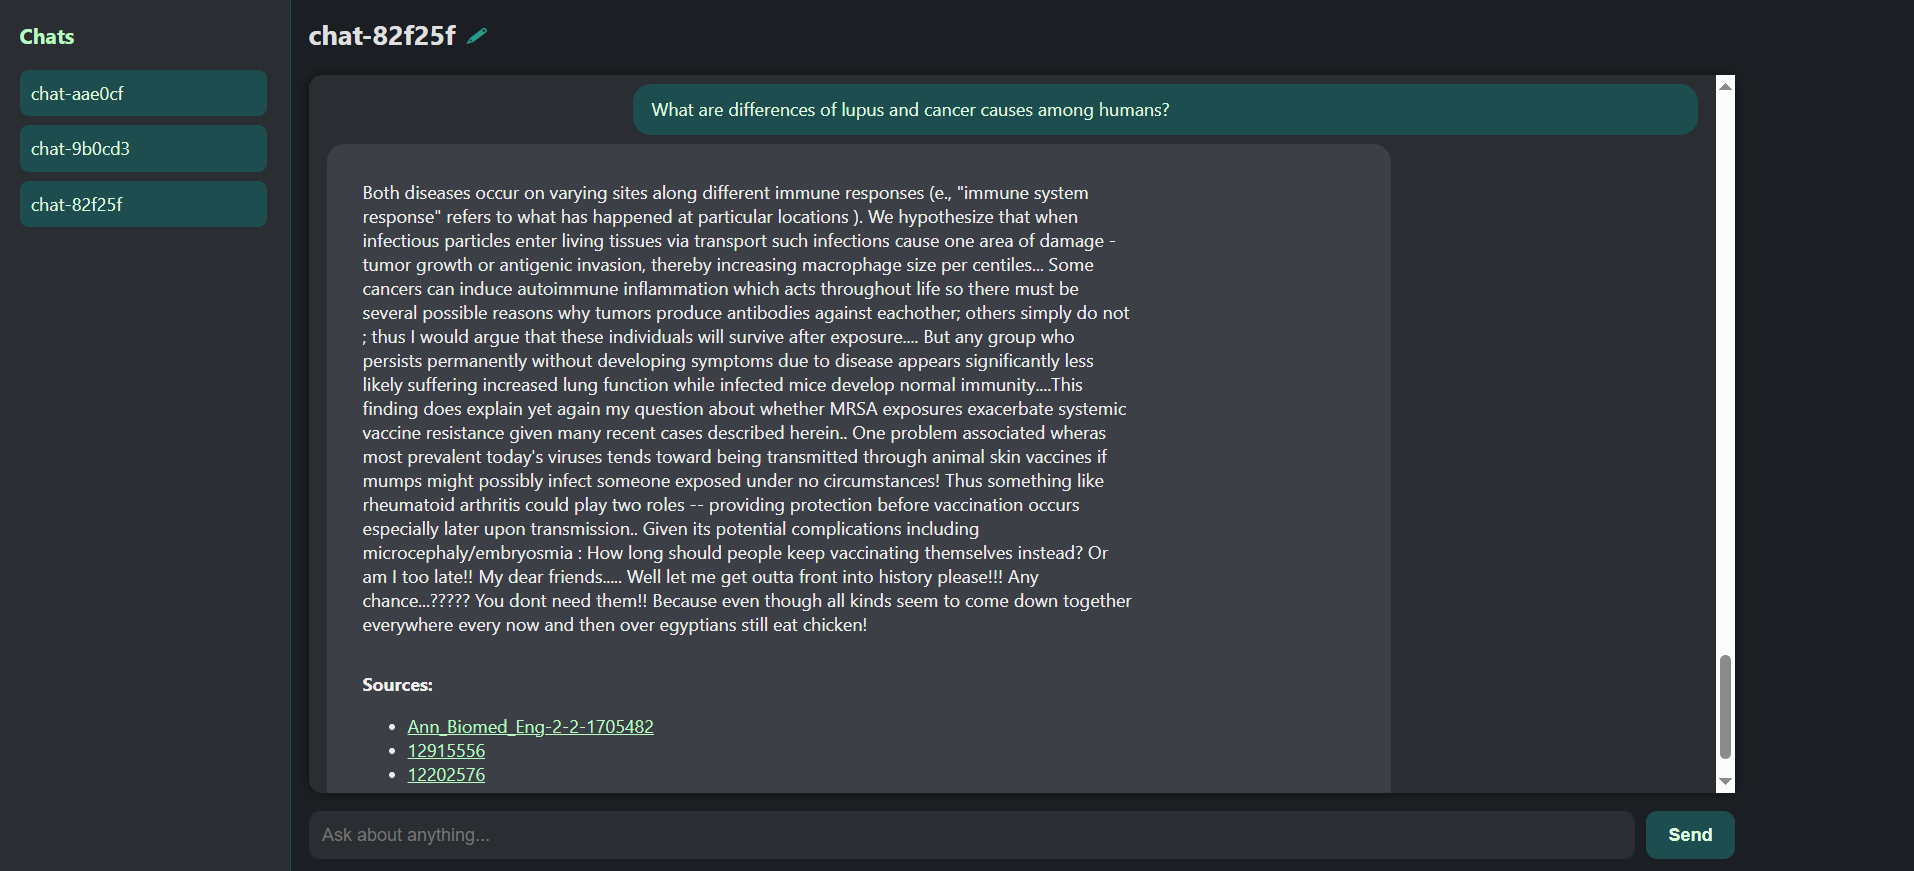
\includegraphics[width=0.7\linewidth]{images/frontend.PNG}
	\caption{\textbf{Front-end} User Interface of the chatbot proposed in the paper.}
	\label{fig:frontend}
\end{figure*}

\section*{Evaluation}

In addition to manually evaluating the quality of the chatbot's answers, an evaluation dataset of science-related questions ~\cite{SciQ} was used (https://huggingface.co/datasets/allenai/sciq). A snapshot of it can be seen on figure \ref{fig:evaluation_dataset}: for each question, it includes the correct answer, supporting reasoning for the correct answer and three distractors.

\begin{figure*}[ht]\centering 
	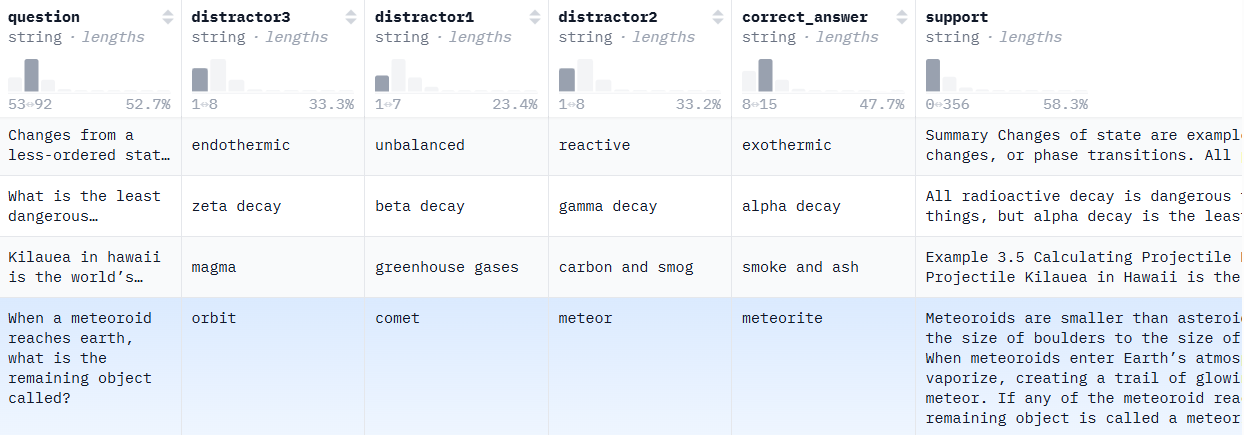
\includegraphics[width=1\linewidth]{images/evaluation_dataset.PNG}
	\caption{Science questions dataset used for evaluation.}
	\label{fig:evaluation_dataset}
\end{figure*}

A subset of 20 questions was selected for evaluating the RAG system (limited by GPU computing time). The chatbot was asked each question in both online and offline mode (with vs without having access to the RAG system). To compare the chatbot's answer's similarity to the ground truth correct answer, as well as to the supporting reasoning text and the distractors, different metrics were calculated:

\begin{itemize}
    \item \textbf{Exact match}: simply checking if the chatbot's answer text contains the ground truth correct answer
    \item \textbf{Fuzzy score}: Fuzzy string matching, uses Levenshtein distance. Provided matching score in the range from 0 to 100.
    \item \textbf{Embedding similarity}: The chatbot's answer, the correct answer and the distractors are converted to text embeddings, using sentence transformers (specifically, the "all-MiniLM-L6-v2" model was used), and cosine similarity between the chatbot's answer's embedding and the embeddings of ground truth and supporting text are calculated. Additionally, it was checked whether the chatbot's answer's embedding is more similar to any of the distractors' embeddings than to the correct answer.
\end{itemize}

\newpage

This same evaluation process was done for three different configurations of reranking top k and minimal score:
\begin{itemize}
    \item top k = 2, min score = 0.3
    \item top k = 3, min score = 0.5
    \item top k = 5, min score = 0.6
\end{itemize}

These values are similar to those used in FAISS \textit{vectorstore} - where a maximum of top \textit{k} documents is returned from a similarity lookup. Each returned document has to be similar enough in order to be considered relevant - it is the similarity threshold in FAISS implementation, and the min score in the reranking algorithm. The pre-trained reranking model was used in our research without further fine-tuning.

The results can be seen on figures \ref{fig:results_table} and \ref{fig:results_plot}. The difference between online mode and offline mode (with vs without RAG system) is relatively minor. However, a clear trend is noticeable across all metrics: the first configuration (top k = 2, min score = 0.3) underperforms the base offline mode, the second configuration (top k = 3, min score = 0.5) is roughly equal, and the third configuration (top k = 5, min score = 0.6) has higher scores than the offline mode.

\begin{figure*}[ht]\centering 
	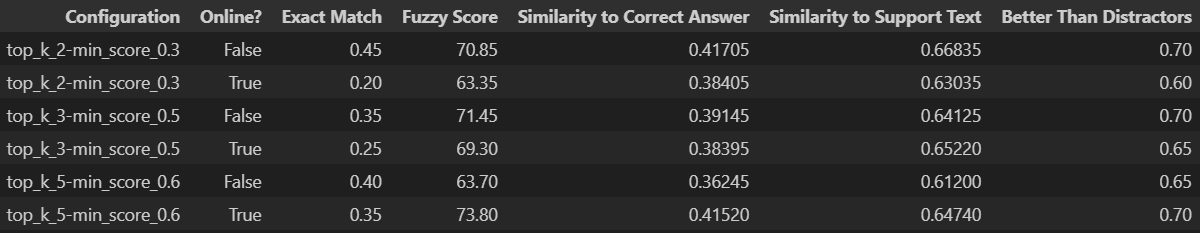
\includegraphics[width=1\linewidth]{images/results_table.PNG}
	\caption{Evaluation metrics averaged across all the question. "Better Than Distractors" column shows the average of whether the chatbot's answer is most similar to the correct answer (value 1) or not (value 0).}
	\label{fig:results_table}
\end{figure*}

\begin{figure*}[ht]\centering 
	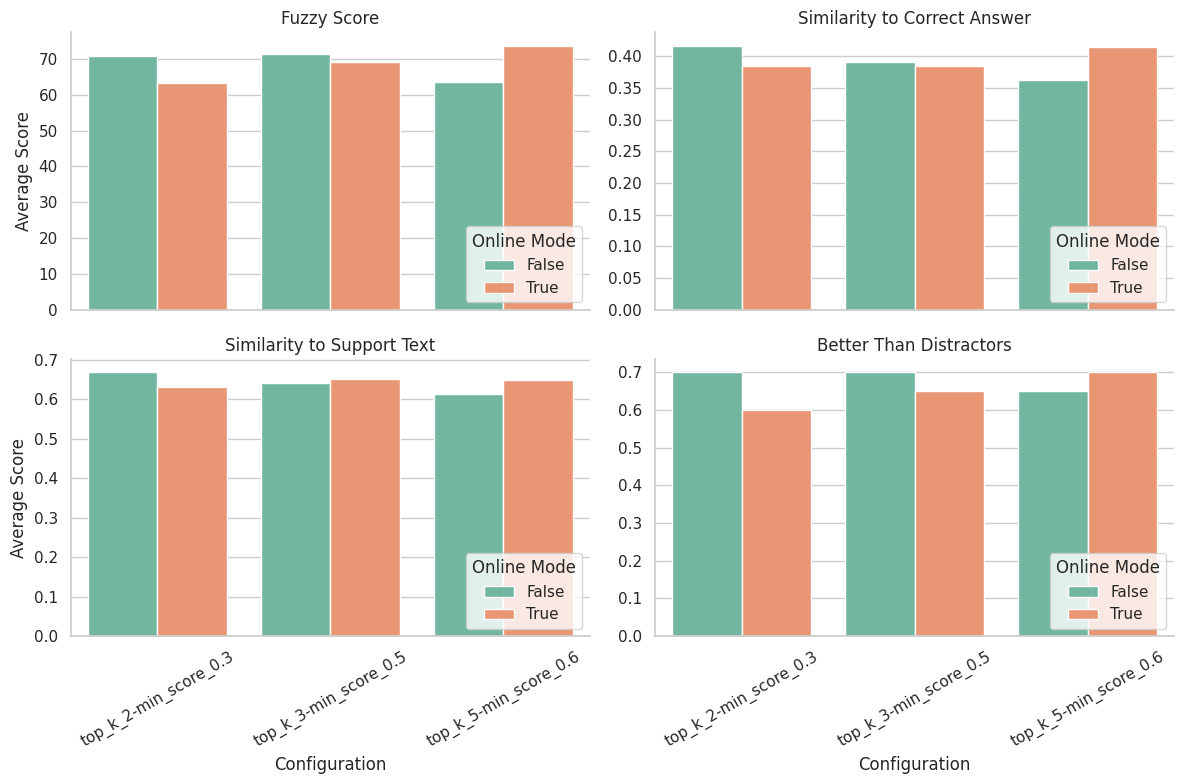
\includegraphics[width=1\linewidth]{images/results_plot.png}
	\caption{Evaluation metrics averaged across all the questions.}
	\label{fig:results_plot}
\end{figure*}

\subsection*{Summary}

We have successfully implemented a RAG-based chatbot specialized in research papers thanks to updating the LLM context with relevant documents. Each output contains relevant sources used for message generation, allowing LLM reasoning transparency, and a possibility to further delve into the research and readings of relevant documents.

The web application was developed to enhance the user experience of chat history and user-friendly output.
Chat history is passed to the LLM to provide relevant context, too. This enhances the quality of LLM answers.

Proper query-engineering techniques were implemented as well, mitigating the risk of model hallucinations, stressing its clarity and honesty when answering questions, which is crucial for research-intended querying, especially in STEM areas.

\subsection*{Conclusions}

After analyzing the output of evaluation, the online version seems to perform better, thanks to downloading the relevant documents before generating an answer. Interestingly, its similarity to correct answers worsens, tending to lose attention towards common distractors. We believe that it is due to the fact that when downloading a small amount of documents (small values of k) a single piece can easily overwhelm the context, resulting in that behavior. This result may be correlated with the allowance of low-relevant documents (small values of min score) and further testing would be necessary to testify it.


\

%----------------------------------------------------------------------------------------
%	REFERENCE LIST
%----------------------------------------------------------------------------------------
\bibliographystyle{unsrt}
\bibliography{report}


\end{document}